%%%%%%%%%%%%%%%%%%%%%%%%%%%%%%%%%%%%%%%%%
% Stylish Article
% LaTeX Template
% Version 1.0 (31/1/13)
%
% This template has been downloaded from:
% http://www.LaTeXTemplates.com
%
% Original author:
% Mathias Legrand (legrand.mathias@gmail.com)
%
% License:
% CC BY-NC-SA 3.0 (http://creativecommons.org/licenses/by-nc-sa/3.0/)
%
%%%%%%%%%%%%%%%%%%%%%%%%%%%%%%%%%%%%%%%%%

%----------------------------------------------------------------------------------------
%	PACKAGES AND OTHER DOCUMENT CONFIGURATIONS
%----------------------------------------------------------------------------------------

\documentclass[fleqn,10pt]{SelfArx} % Document font size and equations flushed left

\setlength{\columnsep}{0.55cm} % Distance between the two columns of text
\setlength{\fboxrule}{0.75pt} % Width of the border around the abstract

\definecolor{color1}{RGB}{0,0,90} % Color of the article title and sections
\definecolor{color2}{RGB}{0,20,20} % Color of the boxes behind the abstract and headings

\newlength{\tocsep} 
\setlength\tocsep{1.5pc} % Sets the indentation of the sections in the table of contents
\setcounter{tocdepth}{3} % Show only three levels in the table of contents section: sections, subsections and subsubsections

\usepackage{lipsum} % Required to insert dummy text
\usepackage[round]{natbib}

%----------------------------------------------------------------------------------------
%	ARTICLE INFORMATION
%----------------------------------------------------------------------------------------

\JournalInfo{GIS Algorithms, January, 2014} % Journal information
\Archive{Research Project, Version 1.0 } % Additional notes (e.g. copyright, DOI, review/research article)

\PaperTitle{Spatial Evolving Agents\\ { \em An heuristic approach in Agent-Based and cellular automata modelling for finding optimal solutions in a geographic context} } % Article title

\Authors{Juan M. Escamilla-Molgora\textsuperscript{1}*} % Authors
\affiliation{\textsuperscript{1}\textit{Department of Physical Geography and Ecosystem Science, Lund University, Sweden}} % Author affiliation
%\affiliation{\textsuperscript{2}\textit{Department of Chemistry, University of Examples, London, United Kingdom}} % Author affiliation
\affiliation{*\textbf{Corresponding author}: molgor@gmail.com} % Corresponding author

\Keywords{Agent-Based Models, Genetic Algorithms, Spatially Explicit Models, GIS Algorithms, Swarm Intelligence, Optimization Heuristics} % Keywords - if you don't want any simply remove all the text between the curly brackets
\newcommand{\keywordname}{Keywords} % Defines the keywords heading name

%----------------------------------------------------------------------------------------
%	ABSTRACT
%----------------------------------------------------------------------------------------

\Abstract{The aim of this review is to describe briefly two related heuristic methods for modelling and simulating spatial phenomena using geographic information systems.
These methods are: {\em Cellular Automata} (CA) and {\em Agent-Based models} (ABM).
An introduction explaining the basic concepts,the {\em rules} and how they work is explained in the fist section. A brief introduction to genetic algorithms is presented in the second part. This exposition would serve as a background for understanding how these models can be used to solve complex problems. Specially problems that defined in an analytical or numerical manner could have a non polynomial time solution.
Finally two iconic examples are given that support the proposed approach. The Axelrod model for cultural aggregation and an ecological application that models the change of vegetation coverage using cellular automata.}

%----------------------------------------------------------------------------------------

\begin{document}

\flushbottom % Makes all text pages the same height

\maketitle % Print the title and abstract box

%\tableofcontents % Print the contents section

\thispagestyle{empty} % Removes page numbering from the first page

%----------------------------------------------------------------------------------------
%	ARTICLE CONTENTS
%----------------------------------------------------------------------------------------

\section{Introduction} % The \section*{} command stops section numbering
In the GIS world there are many different definitions of models. In this review, model would be defined as a simplified representation of reality. A model can be constructed as a computer program that uses a simplified representation of one or more aspects of reality. This attributes are transformed in order to create a new representation of the real-world.
Models can be classified as {\em static}: if the input and output correspond to the same point in time. Or {\em dynamic}: if the output represents a later point in time than the input \citep{longley2005}. Modelling can serve a number of purposes. {\em Static} models provide indexes or indicators that can provide some predictors of impacts, sensitivities, or vulnerabilities. {\em Dynamic} models go further by attempting to project quantifiable impacts into the future and are used to assess different management or development scenarios \citep{abm_prin_conc}. 

An automaton is a processing mechanism with features that change over time based on some internal rules. Automata process information from their surrounding as input. and their characteristics are altered according to rules that govern their reaction to those inputs \citep{abm_prin_conc}. In the scope of this review, {\em dynamic models} would be exemplified as {\em Cellular Automata} or {\em Agent-Based Models}.

\subsection{Cellular Automata}
Cellular automata are dynamical recursive models that are discrete in space, time and state. A simple cellular automata $A$ is defined by a lattice $L$, a state space $Q$, a neighbourhood $N$ and a local transition function $f$ (decision rule) \citep{adamatzky1994}.
$$A = ( L, Q, N, F) $$
Each element (cell) in the lattice $L$ is set in a state $s \in Q$. The cells can be linked in several ways, the most common is a geometric link. Meaning that two cells are connected if they share a common boundary. The cells are indexed by $i \in I$ where $I$ is the index set. Cells change its state in discrete time. The most common case is synchronously, meaning that all cells change their states simultaneously. 
The change in state of cell $c$ depends on the cells that are {\em inside} the neighbourhood $N$ of the $c$ ($N(c)$) and the corresponding transition function $f(N(c))$.
For spatial (geographic) models, two-dimensional C.A. are used. For many applications, a simple neighbourhood of shape 3x3 is used for each cell \citep{Balzter1998}. The neighbourhood that consists of 8 cells surrounding the central cell is called {\em Moore Neighbourhood}. The neighbourhood that have only 4 cells {\em North, South, East, West} is called $Von-Neuman Neighborhood$ \citep{adamatzky1994}. 

C.A. can be $deterministic$ if the change of state in any cell is always the same given the neighbourhood. Contrary, a C.A is $stochastic$ if each cell has a probability of change from one state to another \citep{Balzter1998}. In general, a deterministic C.A. is a type of convolution. 
The transition function $f(N(c))$ also called {\em rules} has the form:
$$a_{t+1}^{c} = f(a_{t}^{c-r},...,a_{t}^{c},...,a_{t}^{c+r})$$
Where: 
$a_{t}^{c}$ represents the state of cell $c$ at time $t$, $r$ is the neighbourhood $c$ and $f$ is the local transition function that represents the transition rules. For each time step $t$ the set $\{a_{t}^{c} | \forall s \in I \}$ is frequently called the configuration of the C.A. at time $t$ \citep{Balzter1998}.
The iconic example of a two dimensional deterministic, nonetheless, chaotic (susceptible to initial conditions and non periodic patterns \citep{devaney2003}) is Conway's Game of Life in which the transition rule depends only whether there exists a constant number of $active$ cells in the neighbourhood see \citep{gardner1971}


\subsubsection{more about transition functions}
Consider a Neighbourhood $N$ of size 3 and a state space $Q = \{0,1\}$, for a one-dimensional C.A. The transition function is going to take as input a boolean vector of size 3. Therefore, the domain will be the $2^3 = 8$ in size. Now, for the output, the function will return $0$ or $1$, meaning that the total number of rules is size $2^8 = 256$. It can be seen that the number of rules or transition functions increases exponentially depending on the size of the neighbourhood. Finding a optimal transition rule for a particular problem often yields to a NP-Complete problem. Several heuristics methods involving fitness measures exists and genetic algorithms is an approach often used \citep{mitchell_ga}. Perhaps the more detail description of cellular automata, specially the 256 rules of the elementary 1-D automaton is the book {\em A new Kind of Science} \citet{wolfram02}.
\subsubsection{Remarks on automata}
The C.A. can represent only the changes in state of the phenomena observed (objects). C.A. can be a good approximation to reality when the abstraction entity is something that does not interact with the object itself. Sometimes it is necessary that the objects transform the environment, and dialectically, the environment affects the response of the objects. For model this type of problems Agent-Based Models are proposed.

\subsection{Agent-Based Models}
Although there is no general consensus on a formal definition of the term $agent$ . There are several characteristics that an Agent-Based Model should have (taken from \citet{abm_prin_conc}):
\begin{itemize}
\item [Autonomy] Agents are independent units capable of process and share information between other agents without the influence of a centralized control.
\item [Heterogeneity] Agents can be defined with distinct characteristics.
\item [Active] Agents are active because they interact with the environment and share the unique characteristics (heterogeneity) in the simulation. Active features involves:
\begin{itemize}
\item[Pro-active]
Agents have goals to achieve based on their behaviours'. For example, agents that try to find a certain path in the space.
\item[Reactive]
Agents can have knowledge of their surroundings. Agents can have also prior knowledge or memory maps. Extending the example, the agents can have prior knowledge of the space, in which direction is the path.
\item[Interactive]
Agents have the possibility to share information between other agents. Agents can query other agents and the environment in an arbitrary size neighbourhood.
\item[Mobile]
Agents can have motility in the space.
\item[Adaptable]
Agents can be designed to modify their inner state based on the environment and the relations with other agents, permitting agents to adapt with a form of memory or learning. Agents can adapt at the individual level (e.g. learning alters the probability distribution of rules that compete for attention), or the population level (e.g. learning alters the frequency distribution of
agents competing for reproduction).

\end{itemize}


\end{itemize}
Agents can also be designed to be adaptive, which can produce Complex Adaptive Systems (CAS; Holland, 1995). In this sense, the agents look for the best suitable conditions, based on their proper characteristics. Using the property of heterogeneity, mentioned before, it is possible to generate many agents with slight variations and make an {\em artificial selection} of the sub-population that fits best certain wanted characteristics. 

\subsection{Genetic algorithms}
\paragraph{Why genetic?} {\em Artificial Selection} is the process in which humans selects members of a biologic population with certain features and make hybrids between the members this sub-population. Generation after generation better individuals emerge from this population. A good example of artificial selection are the dog breeds. Each breed have been raised accordingly to achieve a goal. Better muscle mass, good for hunting, vermin picker or even just for petting. 
A similar process have been abstracted into the machine learning and optimization methods. The process consist of instantiate similar but not identical agents. Define a fitness measure that is a function that assess how the agent's responses to the environment. During the process, a subset of the population with the best fitness values is filtered. Variations, called {\em mutations} are induced into this population.The sub-population reproduce among itself making a new population of siblings.The process is repeated again until the remaining population's fitness gets a high value. 

\subsubsection{The chromosome}
Every agent have intrinsic methods that sense the environment in a certain way and responds according to these factors. This response is called $behaviour$. Each agent can have different $behaviours$ that correspond to different configurations of the sensed space. The set of all $behaviours$ for a given sensed space is called chromosome. 

For example suppose that the agent is a car and the problem to model is to avoid collisions with other cars. The agent sense the environment within a radius of 5 meters. Supposing that the model is implemented in a raster of 1 meter resolution, the number of cells in a radius of 5 meters is 100. Now, suppose that each cell could be either occupied or not. All the sensed input is evaluated using the decision function that outputs either 0 or 1 if cell would be occupied or not the next time step. The chromosome would be the set of all the $2^{100}$ $behaviours$. As in C.A. the sensed space could be indexed accordingly to fit the binary representation of an integer. Therefore, a complete chromosome could be seen as a binary string of size $2^{100}$.
 
The simplest form of genetic algorithm involves three types of operators: {\em selection, crossover (single point), and mutation (after \citep{mitchell_ga})}. 
\begin{itemize}
\item {\em Selection} This operator selects chromosomes in the population for reproduction. The fitter (using the fitness measure) the chromosome, the more times it is likely to be selected to reproduce.
\item {\em Crossover} This operator randomly chooses a locus and exchanges the subsequences before and after that locus between two chromosomes to create two offspring. For example, the strings 11000100 and 11111111 could be crossed over after the third locus in each to produce the two offspring 11011111 and 11100100. The crossover operator roughly mimics biological recombination between two single chromosome (haploid) organisms.
\item {\em Mutation} This operator randomly flips some of the bits in a chromosome. For example, the string 00000100 might be mutated in its second position to yield 01000100. Mutation can occur at each bit position in a string with some probability, usually very small (e.g., 0.001).
\end{itemize}
The process executes iterated until a certain fitness threshold is reached.

\section{Reviewed examples}
\subsection{The effect of habitat destruction pattern on species persistence: A cellular model}
\citet{dytham1995} proposed a cellular automaton to model the persistence of two plant species in environments with different patterns habitats. The model assumes that two competing species can only coexist if one is the competitive dominant ({\em species c}) and the other possesses superior dispersal abilities ({\em species d}). There are four possible patch states in his model: patch permanently destroyed; patch empty but available for colonization; patch occupied by species $c$; patch occupied by species $d$. Colonisation has a range of only one patch. The probability of a patch being colonised is higher if more of its direct neighbours contain the species.
Colonizations and extinctions occur during a discrete time-step. For a new colonised patch is not possible to produce offspring. The impact of four habitat destruction patterns in the population was simulated on a grid of 50x50 cells. The model is a $stochastic$ $celullar$ $automata$ defined with a Moore neighbourhood.
Dytham’s results indicate that species’ coexistence heavily depends not only on the amount of available habitat, but also on the destruction pattern. For more details see \citep{Balzter1998} and \citep{dytham1995}.

\subsection{Segregations of culture}
Robert Axelrod in 1997 proposed a simplified agent-based model that described how social entities (modelled as agents) can form clusters with similar features. This model has been an iconic example in agent-based modelling because of its simplicity and the realistic patterns that emerge from this simple rules.   
Each object, named $social$ $entity$, represent a person within a certain urban context. The idea is to discretize the social features of a social entity. For example: political parties affinities,education, yearly income, age, etc. A distance function is proposed to compare similarities between the objects. The $behaviour$ is that objects move in proportion to the distance between them. Performing the same steps in an iterated fashion would yield to a stabilized pattern of clustered agents, where the more similar objects are closer. For a complete description and analysis of this model see \citep{axelrod1997}. 
\addcontentsline{toc}{section}{\hspace*{-\tocsep}Introduction} % Adds this section to the table of contents with negative horizontal space equal to the indent for the numbered sections


%------------------------------------------------

%\section{Methods}
%
%\begin{figure*}[ht]\centering % Using \begin{figure*} makes the figure take up the entire width of the page
%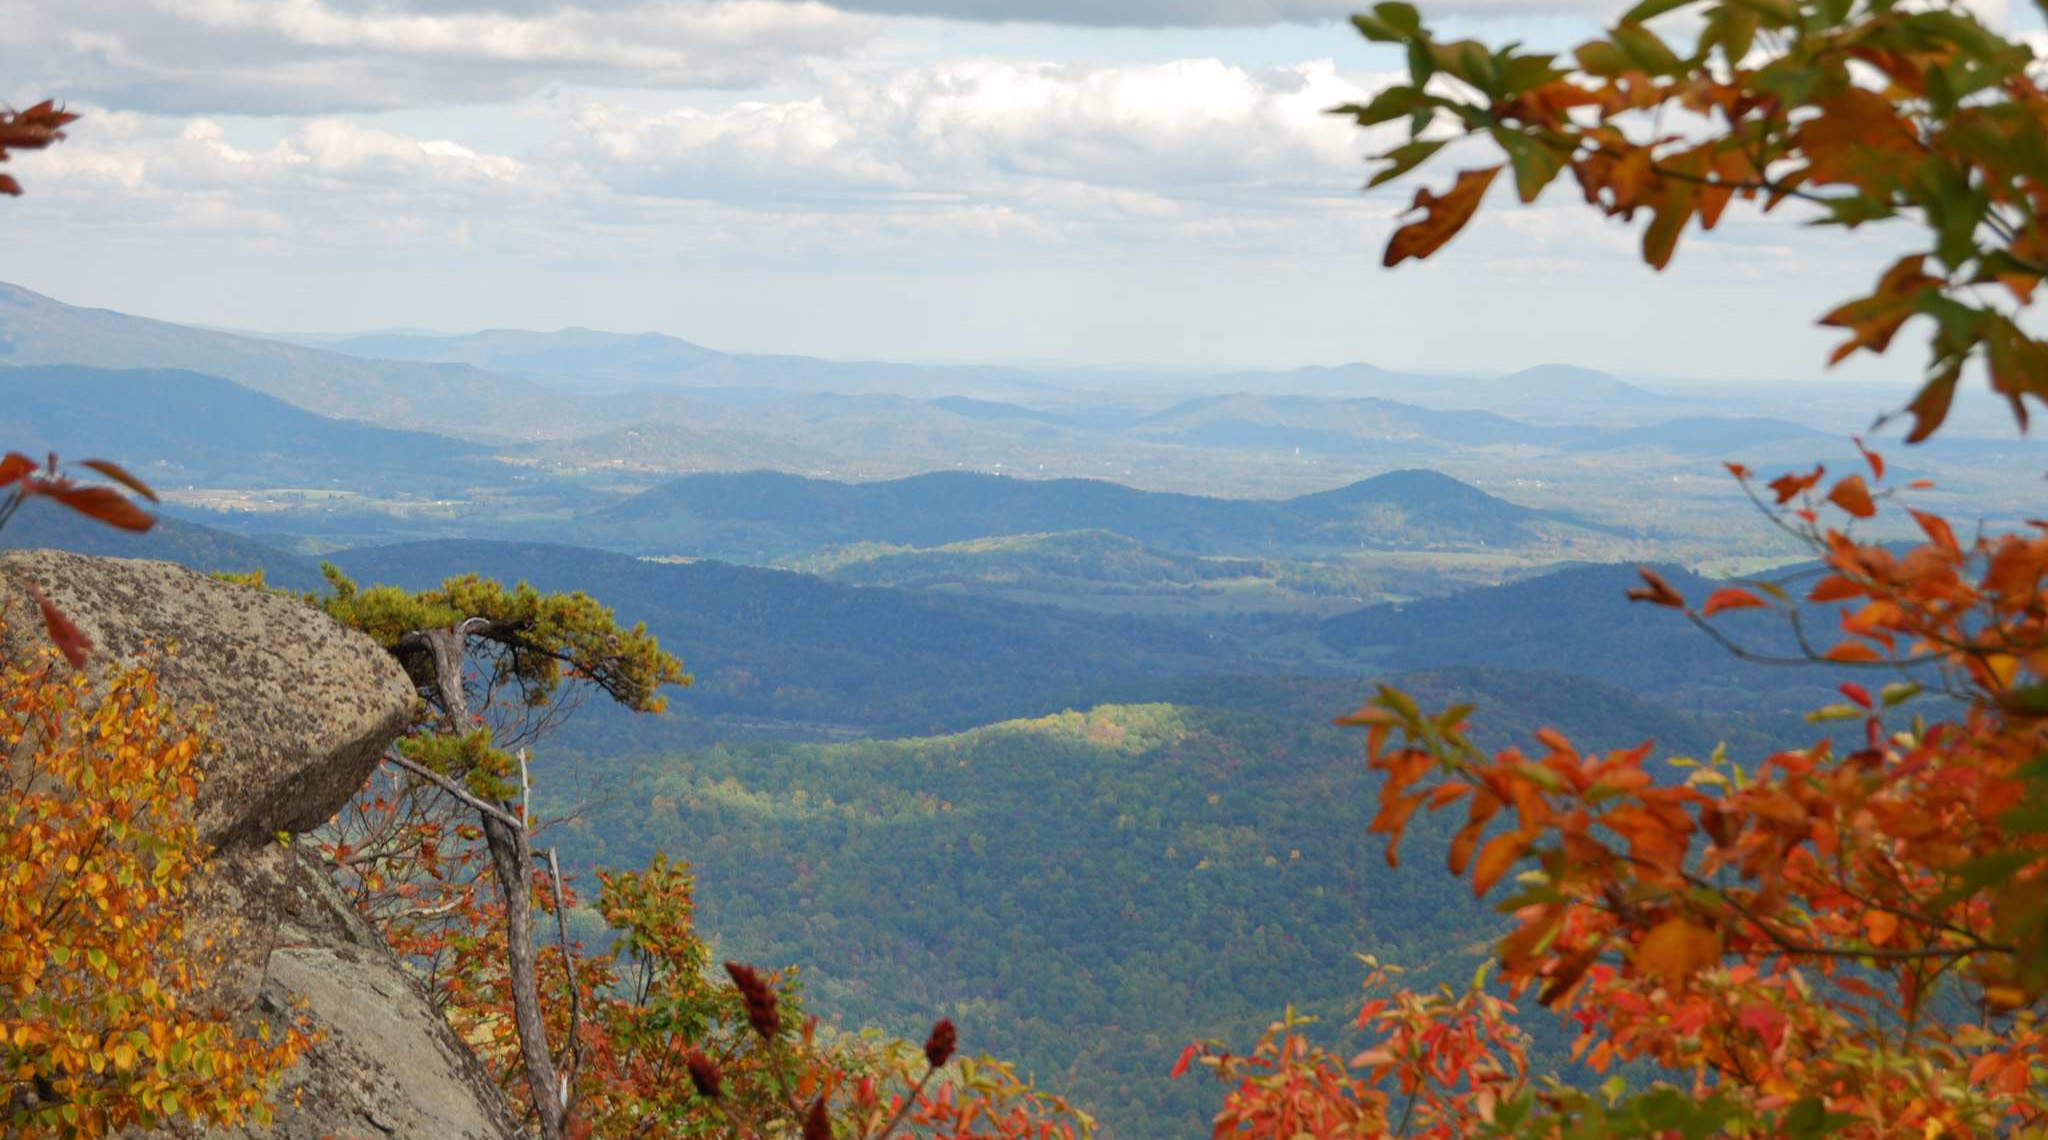
\includegraphics[width=\linewidth]{view}
%\caption{Wide Picture}
%\label{fig:view}
%\end{figure*}
%
%
%\begin{equation}
%\cos^3 \theta =\frac{1}{4}\cos\theta+\frac{3}{4}\cos 3\theta
%\label{eq:refname2}
%\end{equation}
%
%
%\begin{enumerate}[noitemsep] % [noitemsep] removes whitespace between the items for a compact look
%\item First item in a list
%\item Second item in a list
%\item Third item in a list
%\end{enumerate}
%
%\subsection{Subsection}
%
%
%\paragraph{Paragraph} \lipsum[7] % Dummy text
%
%
%\subsection{Subsection}
%
%
%\begin{figure}[ht]\centering
%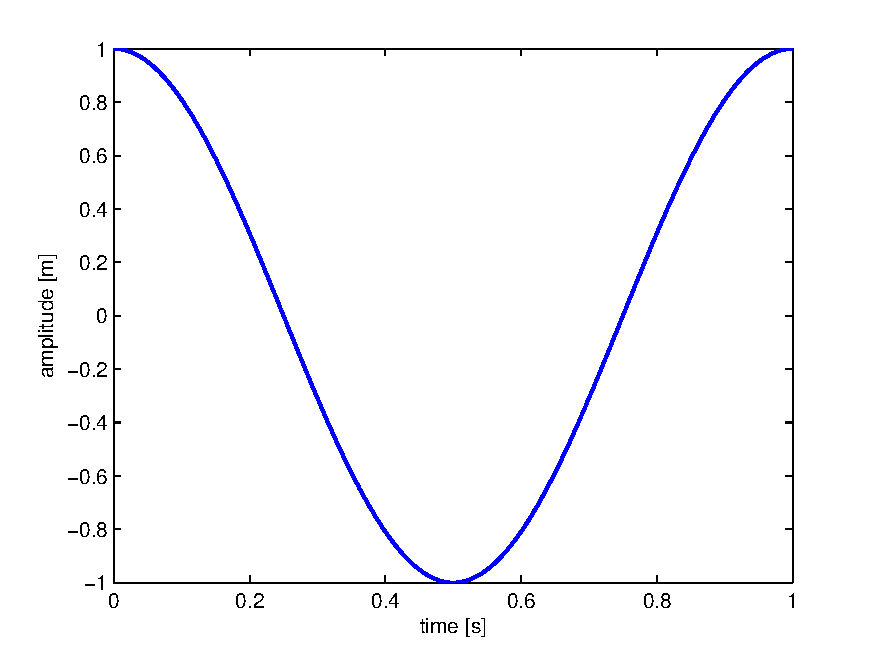
\includegraphics[width=\linewidth]{results}
%\caption{In-text Picture}
%\label{fig:results}
%\end{figure}
%
%Reference to Figure \ref{fig:results}.
%
%%------------------------------------------------
%
%\section{Results and Discussion}
%
%
%\subsection{Subsection}
%
%
%\begin{table}[hbt]
%\caption{Table of Grades}
%\centering
%\begin{tabular}{llr}
%\toprule
%\multicolumn{2}{c}{Name} \\
%\cmidrule(r){1-2}
%First name & Last Name & Grade \\
%\midrule
%John & Doe & $7.5$ \\
%Richard & Miles & $2$ \\
%\bottomrule
%\end{tabular}
%\label{tab:label}
%\end{table}
%
%\subsubsection{Subsubsection}
%
%
%\begin{description}
%\item[Word] Definition
%\item[Concept] Explanation
%\item[Idea] Text
%\end{description}
%
%\subsubsection{Subsubsection}
%
%
%\begin{itemize}[noitemsep] % [noitemsep] removes whitespace between the items for a compact look
%\item First item in a list
%\item Second item in a list
%\item Third item in a list
%\end{itemize}
%
%\subsubsection{Subsubsection}
%
%\subsection{Subsection}
%
%%\lipsum[15-23] % Dummy text
%
%%------------------------------------------------
%
%\section*{Acknowledgments} % The \section*{} command stops section numbering
%
%\addcontentsline{toc}{section}{\hspace*{-\tocsep}Acknowledgments} % Adds this section to the table of contents with negative horizontal space equal to the indent for the numbered sections
%
%So long and thanks for all the fish.

%----------------------------------------------------------------------------------------
%	REFERENCE LIST
%----------------------------------------------------------------------------------------

\bibliographystyle{plainnat}
\bibliography{references}

%----------------------------------------------------------------------------------------

\end{document}